% HA Schema


\chapter{High availability schema}
This chapter explains the High Availability that will be tested through the Thesis. 

\section {Main schema}
There are two servers which we will name the primary one and the secondary one. Each of them are linked by two means. The service link is the main network interface which it's connected via a normal switch. It will serve content to the final users. The communication link, which it's used for the cluster managemente and syncronisation is done via a crossover cable.

We can see the main schema, where we have added two final clients at figure \ref{fig:main-schema}.

\begin{figure}
  \centering
    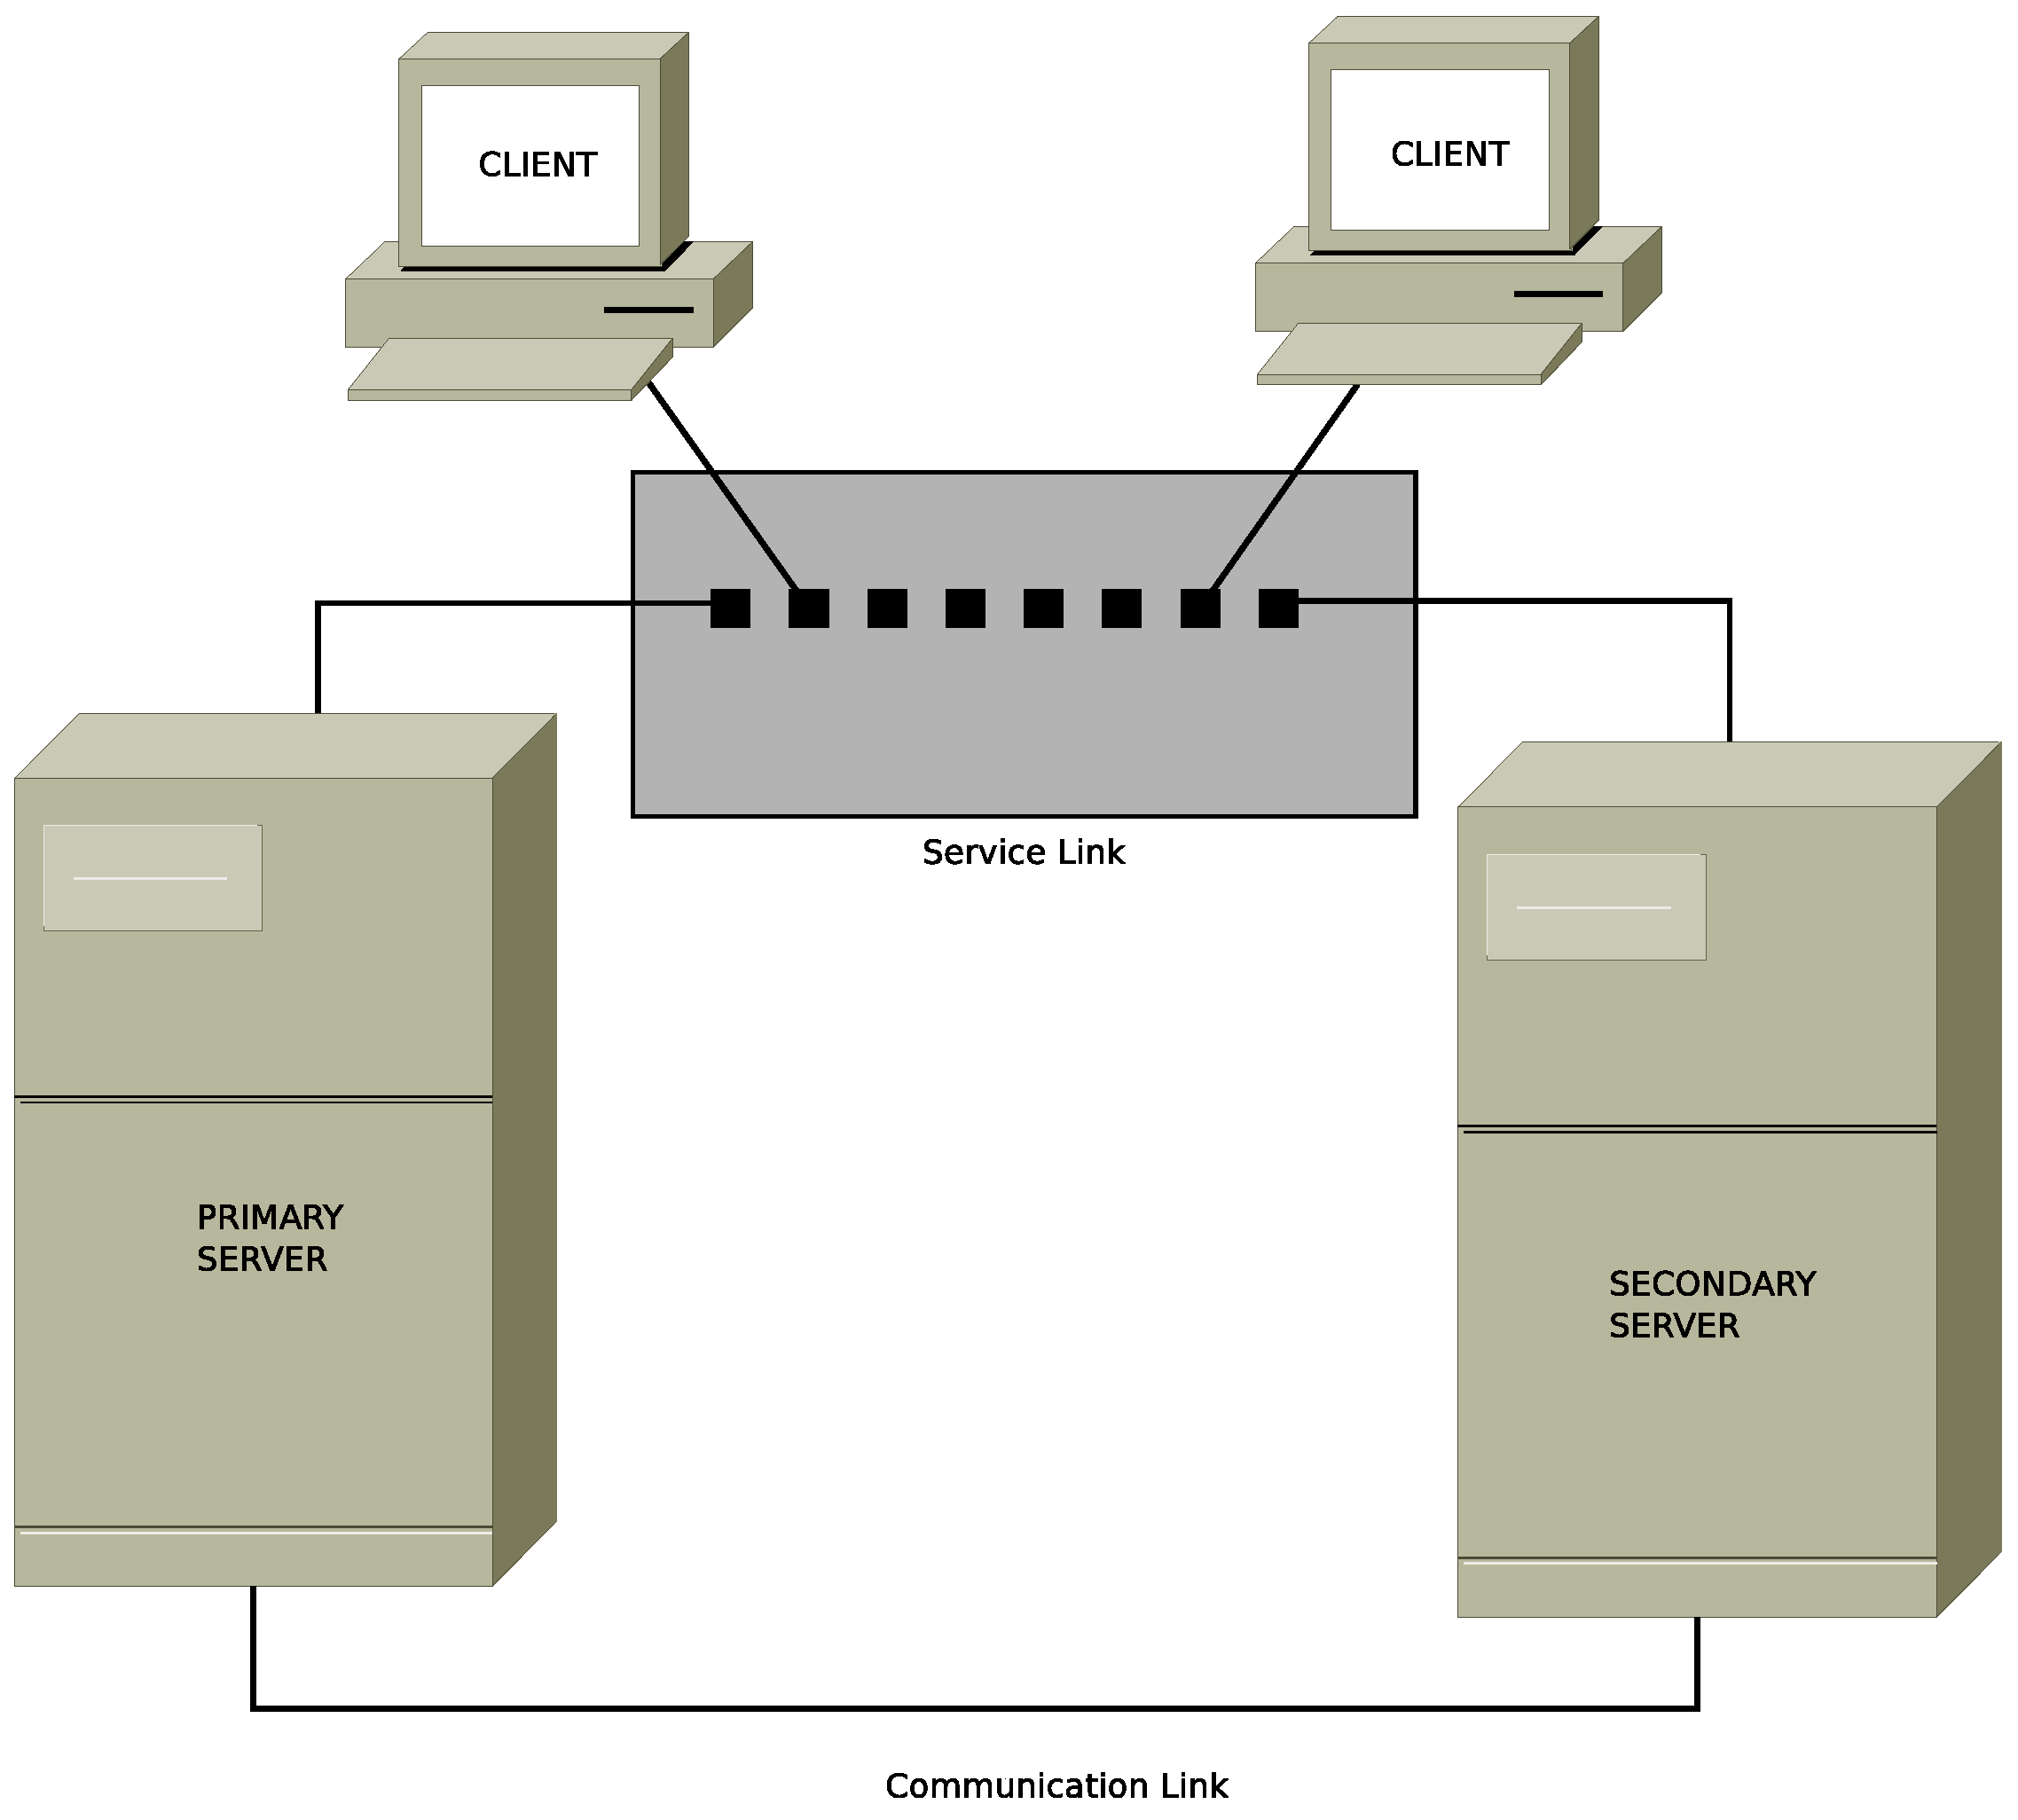
\includegraphics[width=0.8\textwidth]{img/ha_main_schema.eps}
  \caption{High Availability main schema}
  \label{fig:main-schema}
\end{figure}

\section {Primary server}
\subsection {Specifications}
The primary server specifications are as follow:
\begin{itemize}
  \item RAM: 4 GB
  \item Hard disk: 100 GB
  \item Processor: 2 x 2,40 Ghz
\end{itemize}

\section {Secondary server}
\subsection {Specifications}
The primary server specifications are as follow:
\begin{itemize}
  \item RAM: 4 GB
  \item Hard disk: 100 GB
  \item Processor: 2 x 2,40 Ghz
\end{itemize}





